\section{Key-value server}
 Before we get into the details of MS5, we would like to revisit the implementation of the distributed key-value storage system we were tasked to develop and briefly discuss some of its features. Figure \ref{fig:ms4_arch} displays how a client interacts with its Connection Handle Thread (CHT), the helper thread assigned to serve it. In the following sections, we take a deeper look at how the client side and storage system visible in \ref{fig:ms4_arch} are structured and how they function.

\begin{figure}[h]
	\centering
	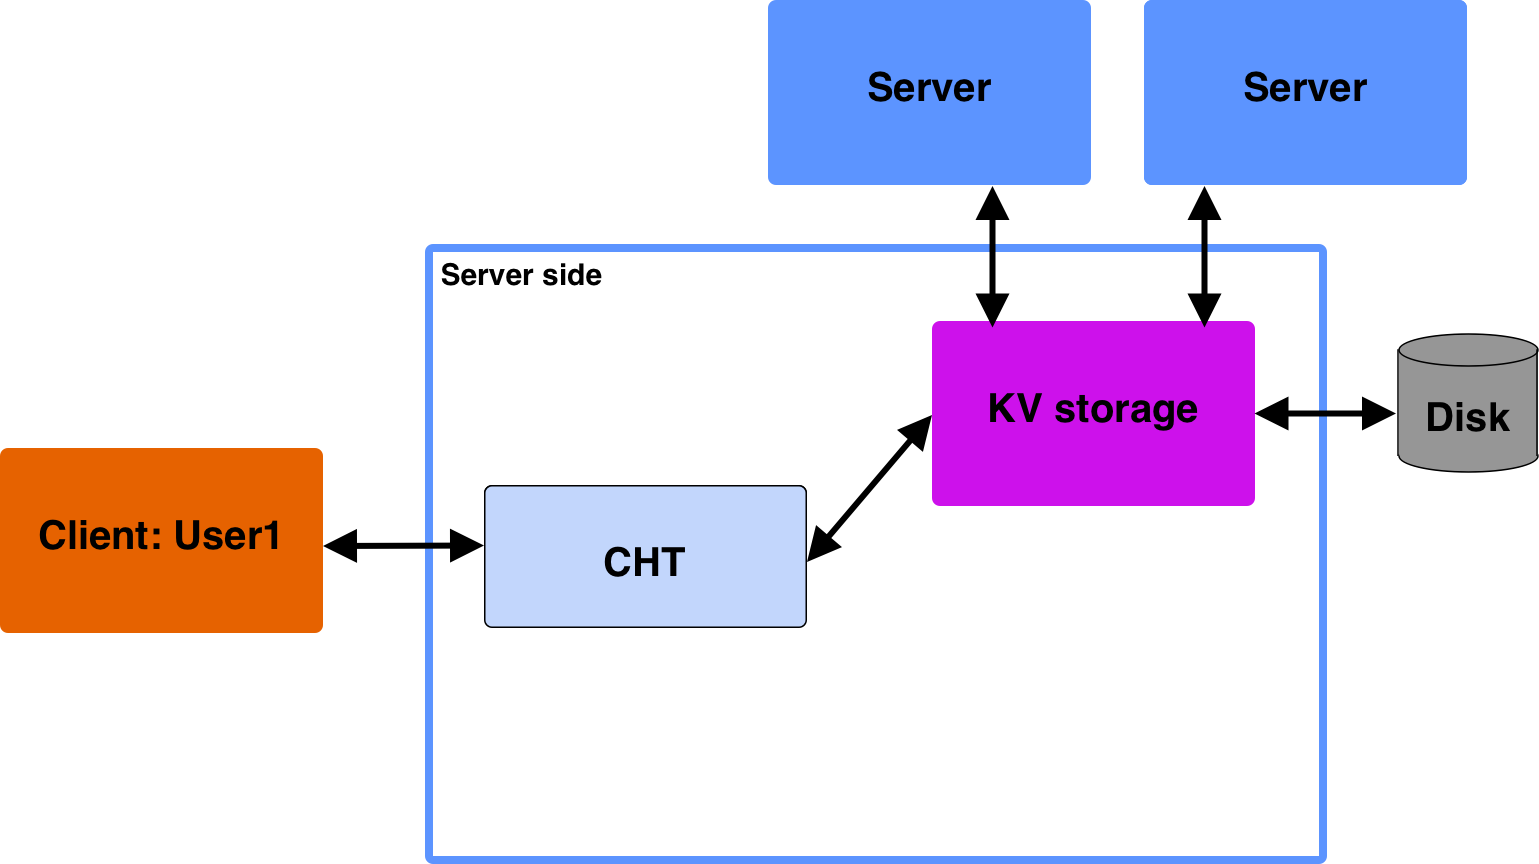
\includegraphics[width=\linewidth]{figures/kvserver/ms4_structure.png}
	\caption{Key-value server architecture}
	\label{fig:ms4_arch}
\end{figure}



%Client Side
\subsection{Client side}

\begin{figure}[h]
	\centering
	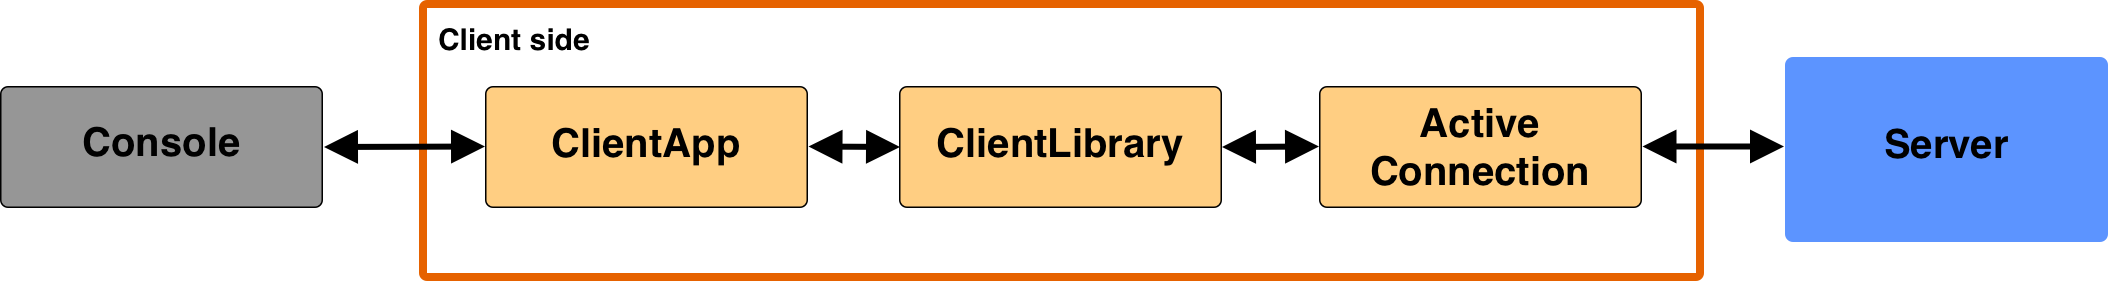
\includegraphics[width=\linewidth]{figures/kvserver/client_arch.png}
	\caption{Client side architecture}
	\label{fig:client_arch}
\end{figure}

The client side consists of the three following main components as seen in figure \ref{fig:client_arch}:

\begin{enumerate} 
  \item \textit{ClientApp}: represents the client interface which allows input through the console. From there the client is able to issue commands to connect to and disconnect from the system, interact with the key-value store and chat. The input is then checked and parsed before getting sent to the ClientLibrary. The result of the user's request gets displayed on the console through the ClientApp.
  \item \textit{ClientLibrary}: serves as a bridge between the client and the server. It contains an instance of the hash ring and is responsible to connect to the correct server.
  \item \textit{ActiveConnection}: abstracts the TCP socket connection to the server which allows the client to exchange data with the CHT without worrying about the underlying structure.
\end{enumerate}
 
 % Server side
\subsection{Server side}

As previously mentioned, the CHT waits on the socket for the client to send a request. Afterwards, the request is forwarded to the key-value processor (KVP), which parses the client's string and translates it into direct DOPs. Then the ServerRing, which contains information about the hash ring, is called to check whether the current server is responsible for performing the requested operation on the provided key or not. In the former case, the request gets transferred to the KVStore. There, the read operations get passed on to the cache. In case of a cache miss it gets passed further to the DiskStore. Write operations instead are redirected to the cache, the DiskStore and the Replication Manager (RPM). 

Upon starting the server, the DiskStore creates a directory containing three subdirectories. One for storing the keys it has write access to and one for each of the key sets it has only read access to. The second type can be refered as the replica folders. A file inside one of those directories represents a key-value pair with the key being the file name and the value the file content.
The RPM is in charge of both sending updates to the server's replicas and receiving updates sent by the responsible servers.

As in the most DBS there are trade-offs between the properties availability, consistency and partition tolerance.

With Milestone 4, replication is added to the system with the intention of increasing the availability by distributing the data records to the two replica servers. Redundancy comes along with the replication strategy, however when a node crashes or fails, read operations can be processed via replicated servers and after stabilization of the ring be accessed the same way as before.
Our system conforms to the first property of BASE by being generally available, because servers respond to clients requests even if a latency occurs. Furthermore we furfill the CAP Partition by replicatiing the data across multiple servers. Lastly we meet the durability goal of the ACID model since we ensure that by persisting the data permanantly on disk.

Eventual consistency is achieved within the system due to requirements of Milestone 4. If there are no updates for a long time all the replicas will become eventually consistent by updating key ranges of the coordinator and replica nodes placed on an hashring. In order to maintain strong consistency as described in \ref{sec:background_acid}, a client performing a \texttt{PUT} operation would have to also wait until the value gets sent over to both of the servers replicas, which would result in slower \texttt{PUT}s. Since our system is not designed to handle important real-time transactions, such as in a banking system, eventual consistency satisfies our database needs while allowing faster response times and higher availability. 

The group chat extension, later to be discussed thoroughly, preserves the same requirements.

Since the implementation of Milestone 3, it is possible to monitor key-value stores continuously. The ECS pings each key-value server every 700 ms to be informed about the servers’ availability. If a server does not respond to the ping within a given period, it is considered shutdown. With replication active, single failing server nodes can be tolerated, thus partition tolerance is provided as well. Since each piece of data exists on three different servers, the only way information can get permanently lost is if all three responsible servers crash simultaneously with no time in between to transfer data to a running server.


